%!TEX root = thesis.tex

\chapter{Body Part Detection}
\label{ch:bodyparts}

To perform hand pose estimation of a person in a image, hands need to be localized in the image first. Hands are very can have different appearances and different orientations this is a very difficult task. Also hand size and shape but also skin color are different per person. One way to localize the hands is by searching for skin like colors in an image given that this color profile is known. A generic skin color model based on average skin color has been constructed for this purpose\cite{Jones1999}, but this method is sensitive for error when the skin is colored by a light source. It would be much better to have a method for obtaining the skin color of the hands from a image itself. This can be done by extracting the a skin model from a face, which is much easier to detect.

\section{Building a skin model}
\label{sec:skinmodel}

\subsection*{Face localization}

\begin{figure}
  \center{}
    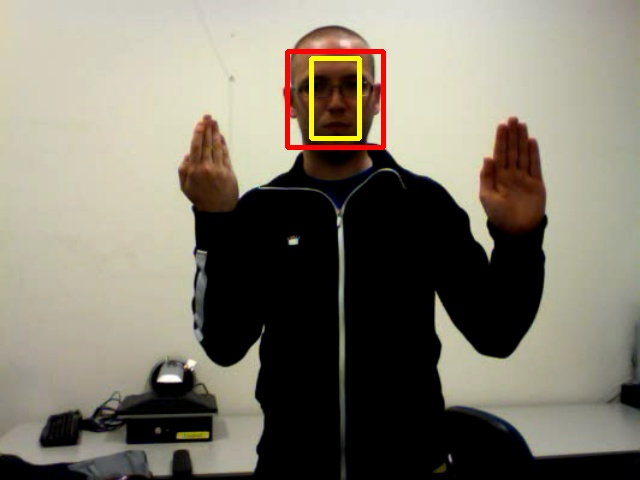
\includegraphics[width=0.3\textwidth]{figures/pipeline/detected.jpg}
  \caption{Face detection}
  \label{fig:face_detection}
\end{figure}


Finding faces in a image is a rather well solved problem. Faces are easy to detect, since it has easy to detect features like eyes, eyebrows, a mouth and a nose. When comparing different faces, these features are \- with a small variation \- on the same distance and orientation. Also people don't tilt their head often, or not more than a couple degrees. Face detection can be done in a fast and robust way using a haar classifier, a boosted rejection cascade that is trained with Haar\-like wavelet\cite{Lienhart2002}. This is a method for detecting faces that doesn't rely on color information. The classifier is run over the image on different scales, and positions with a score above a certain threshold are classified as face position.  Using a haar classifier to search for a face and obtain a skin color profile has been done before with the lab color space \cite{Stenger2006}, but in this case the HSV color space is used.


\subsection*{Color space conversion}

\begin{figure}
  \center{}
    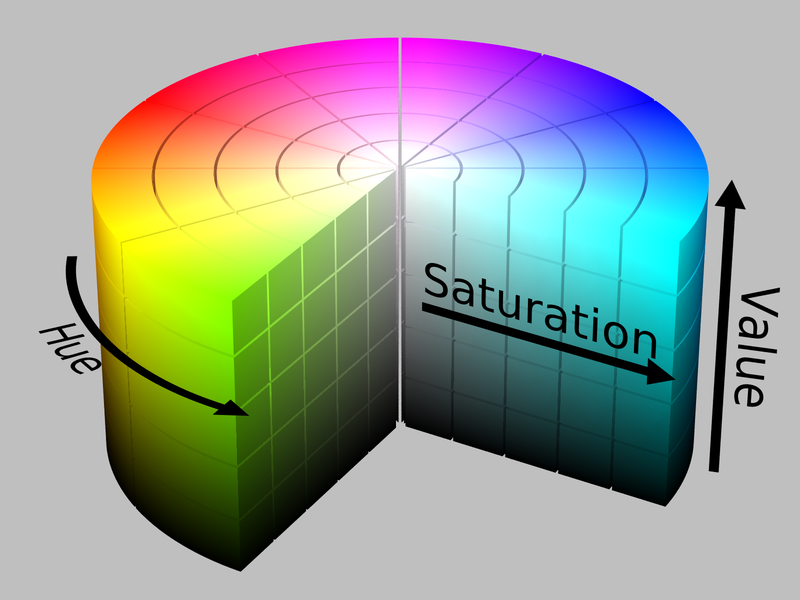
\includegraphics[width=0.3\textwidth]{figures/hsv.png}
	\caption{The Hue, Saturation, Value color space}
	\label{fig:hsv}
\end{figure}

Usually, pixel values of a image are stored in the Red, Green Blue (RGB) color space where specific colors can be represented with combinations of these primary colors. A more intuitive color space is Hue Saturation Value (HSV), which comes closes to how humans perceive color. The hue (color) from Saturation (how concentrated the color is) and from Value (brightness) HSV When a subject is lighted by a light source with uniform hue distribution, the light doesn't change the hue or saturation of the subject. The only thing that will change is the intensity, which is changing because of the light source's intensity, distance or (self casted) shadow. Since we want to extract hand pixels independent of the illumination intensity, we can ignore this channel and only use the hue and saturation.

As many things in computer vision in theory this should work, but in practice it doesn't or not perfect. A light source never has a uniform distribution and \emph{will} color the subject. But in our case that doesn't matter, since all skin pixels in the image will have the same shift in the hue spectrum.

The RGB color space is transformed into the HSV color space using the following equations:
\begin{eqnarray*}
  V & \leftarrow & \max(R,G,B) \\
  S & \leftarrow & \left\{
  \begin{array}{l l}
    \frac{V-\min(R, G, B)}{V} & \quad \text{if $V \neq 0$} \\
    0 						  & \quad \text{otherwise} \\
  \end{array} \right.\\
  H & \leftarrow & \left\{
  \begin{array}{l l}
    \frac{60(G - B)}{S}     & \quad \text{if $V = R$} \\
    \frac{120 + 60(B-R)}{S} & \quad \text{if $V = G$} \\
    \frac{240 + 60(R-G)}{S} & \quad \text{if V = B} \\
  \end{array} \right.\\
\end{eqnarray*}


The input 3 channel RGB image is transformed into a 3 channel HSV image, after which the brightness channel is discarded. From the hue and saturation channel together with the face region we can build a histogram which will represent a statistical skin model.

\begin{figure}[htbp]
  \centering
\subfloat[hue channel]{\label{fig:hue}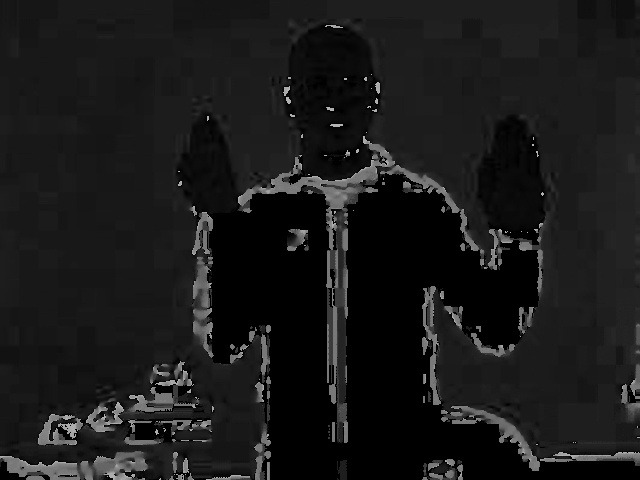
\includegraphics[width=0.3\linewidth]{figures/pipeline/hue.jpg}}
\hspace{0.03\linewidth}
\subfloat[saturation channel]{\label{fig:saturation}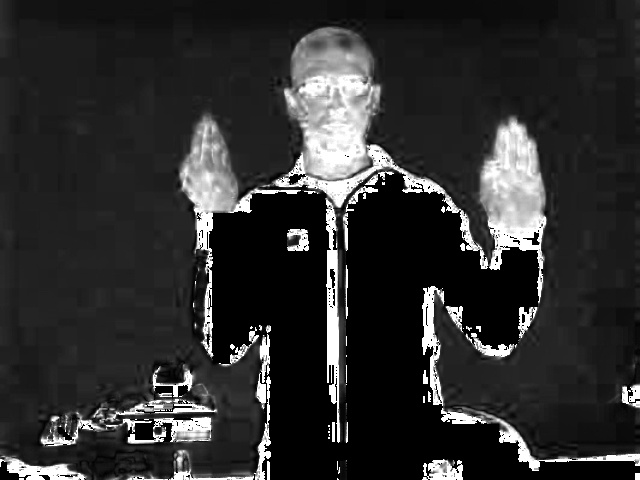
\includegraphics[width=0.3\linewidth]{figures/pipeline/saturation.jpg}}
\hspace{0.03\linewidth}
\subfloat[value channel]{\label{fig:value}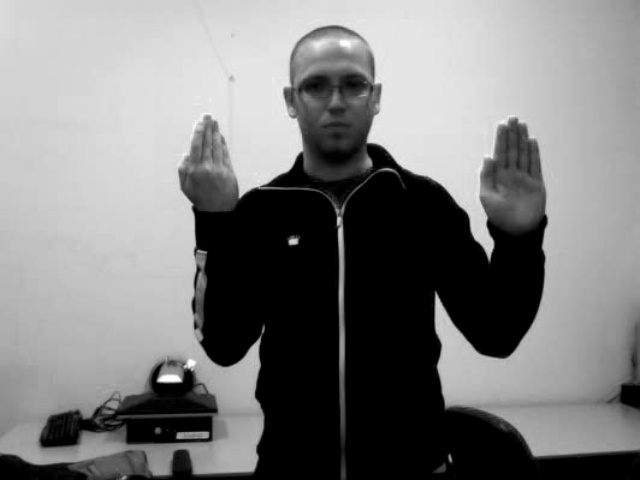
\includegraphics[width=0.3\linewidth]{figures/pipeline/value.jpg}}
  \caption{The HSV channels}
  \label{fig:hsvchannels}
\end{figure}





\subsection*{Skin color histogram}

\begin{figure}
    \center{}
    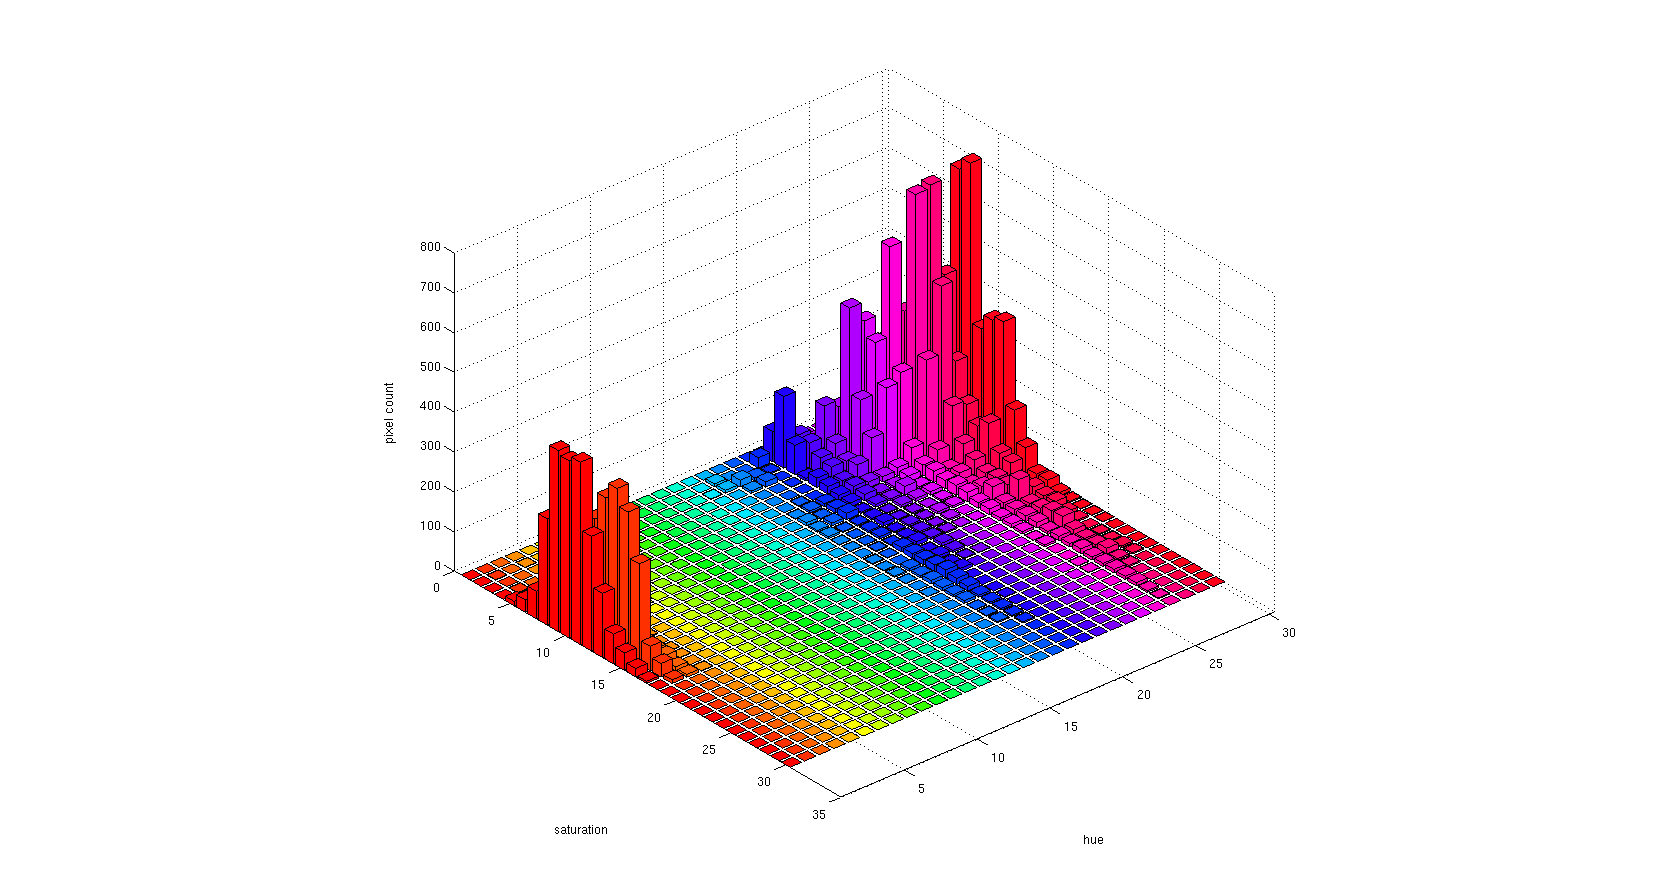
\includegraphics[width=0.5\textwidth]{figures/pipeline/histogram.png}
	\caption{A histogram of face pixels}
	\label{fig:histogram}
\end{figure}


The skin color model is represented in a 2 dimensional histogram, where the first dimension is Hue and the second is Saturation. The histogram is filled with the values from the detected face region. After, the histogram is normalized - all values are divided by the sum of all bins. This makes the histogram independent of the original image size, and each histogram bin value represents a 'skin probablility'.

When all pixels are evaluated, the histogram is normalized - all values are divided by the sum of all bins. This way when all values are added together, the sum will be equal to 1. This makes the histogram independent of the image size, and each value represents a 'skin probability'. \autoref{fig:histogram} is a histogram of face pixels.

\subsection*{Back projection}

\begin{figure}
    \center{}
    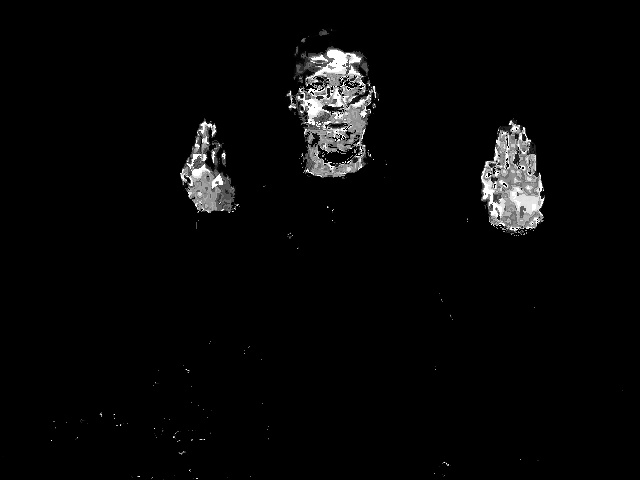
\includegraphics[width=0.4\textwidth]{figures/pipeline/backproject.jpg}
 	\caption{Backprojection}
	\label{fig:backproject}
\end{figure}


A back projection is the combination of an image and a histogram. The result is a new single channel image. All pixels in the input image are iterated and the corresponding bins are looked up in the histogram. The pixel in the same position in the new image is replaced with the value from the histogram. If the histogram is a skin color histogram, the resulting image will have high values for pixels that are skin-like pixels, and low values for other pixels. The result of the process can be seen in \autoref{fig:backproject}.


\subsection*{Threshold}

\begin{figure}
    \center{}
    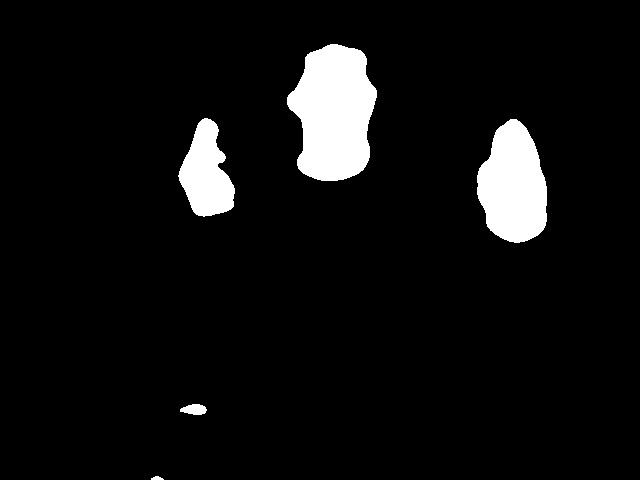
\includegraphics[width=0.4\textwidth]{figures/pipeline/thresholded.jpg}
	\caption{Thresholded image}
	\label{fig:threshold}
\end{figure}


To label pixel to be skin color or not, we need to define a way of doing this automatically. The easiest way to accomplish this is by defining a threshold. All pixel values below a certain threshold are replaced with false or 0, all above this threshold will be replaced with true or 1. This results in a binary image with labels for (non) skin pixels. This introduces one parameter - the threshold for going from the probabilistic domain to the binary domain.

\subsection*{smoothing}


\subsection*{morphological operations}

\begin{figure}
    \center{}
    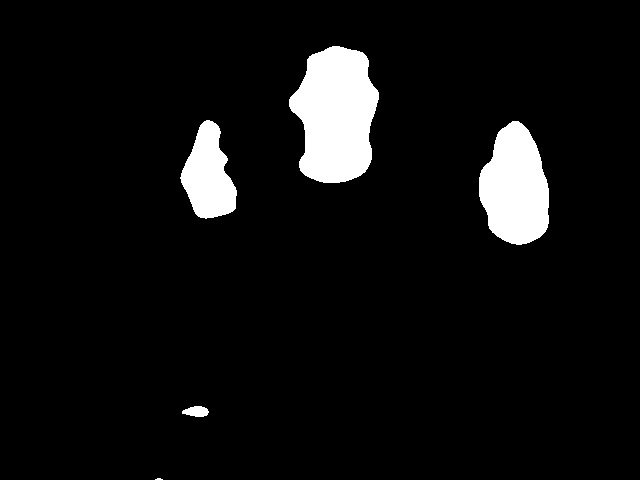
\includegraphics[width=0.4\textwidth]{figures/pipeline/closed.jpg}
	\caption{Morphologically closed}
	\label{fig:closed}
\end{figure}

A morphologic closing operation of A by B is obtained by the dilation of A by B, followed by erosion of the resulting structure by B. The result of performing this operation is that small holes in the binary image are removed, and edges are smoothed.

\section{Object localization}

\subsection*{Pixel grouping, contour extraction}
To be able to say something useful about groups of pixels, one need to know which pixels belong together. This can be done by clustering. In this case clustering is performed by grouping pixels together to touch horizontally and vertically. This is done with the algorithm described in \cite{Suzuki1985}. This algorithm also constructs a list of pixels that form the border of a group. This list of pixels can be used for many interesting things, like finding the top position of the group in a fast way, or to find out if a unidentified pixel is inside the group. Clustering contour extraction\cite{Suzuki1985}.

From the contours of the group a square region of interest can be defined by calculating the outer borders of the group. This window will be called the hand window.

\subsection*{Blob labeling}

\begin{figure}
    \center{}
    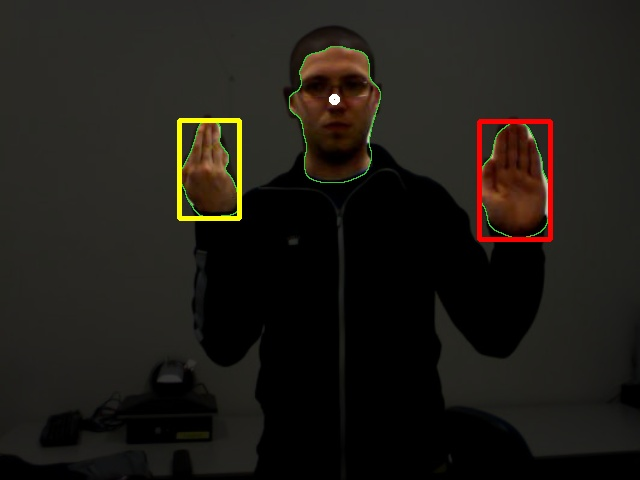
\includegraphics[width=0.4\textwidth]{figures/pipeline/contours.jpg}
	\caption{Labeled blobs}
	\label{fig:contours}
\end{figure}


Now we have grouped skin pixels (blobs) we need to know blob is what body part. It is assumed that there is only one person in the image and that the body is covert with clothing except for the head an hands. In a optimal situation this would result in 3 blobs, 2 for the hands and one for the head. For one blob it is already known what body part it is - the face. In the face detection phase we found a face in the image, so the blob containing the center point of the detected phase is the face blob. Usually the left hand is on the left of the head and the right hand on the right side. If there are 3 blobs, and the face is the middle blob, we labeling is done. But unfortunately in practice this isn't always the case. Often there are more or less blobs, because the background has skin-like color, a hand is difficult to detect or is occluded. Also the order of hands and head can change, a left hand doesn't necessarily need to appear on the left side of a head. In this case some more intelligent decision process. 

First the surface of each blob is calculated and then the blobs are sorted by size. The blob containing the head is removed from the list, since we already know this label. Also very small blobs are removed, because these are probably noise. The removal threshold surface is set to:

\begin{equation}
T = (\frac{h}{20})^2
\end{equation}

All blobs smaller than this value are discarded. 

Assuming the hands or the second biggest skin like objects in the image, the 2 or less biggest blobs are taken from the list and the rest is also discarded. If there is no biggest blob, the labeling is finished - there is only a head in the image. If there is one blob left, the left or right position relative to the head is the hand label. If there are 2 hands, there are 3 possible situations, 1 where the head is in the middle which is already described. If both hands are on the left of the head, the most outer left blob is labeled as left and the other as right. This is visa versa for right.

\begin{algorithm}
\caption{Blob labeling heuristics}
\label{blobheuristics}
\begin{algorithmic}
	\STATE head $=$ left $=$ right $=$ None
	\STATE faceCenter $=$ getFaceCenter()
	\STATE blobs $=$ getContours()
	\STATE limbs $=$ []
	
	\FOR{blob in blobs}
		\IF{blob.contains(faceCenter)}
			\STATE head $=$ blob
		\ELSE
			\STATE blobs.append(blob)
		\ENDIF
	\ENDFOR

	\STATE blobs $=$ sortBySize(blobs)
	\STATE blobs $=$ blobs[-2:]
	\STATE blobs $=$ sortByXPosition(blobs)

	\STATE $n = $ len(blobs)
	\IF{$n == 2$}
	    \STATE left $=$ blobs[0]
	    \STATE right $=$ blobs[1]
	\ELSE
		\IF{$n == 1$}
		    \IF{blobs[0].center[0] $<$ face\_center[0]}
		        \STATE left $=$ blobs[0]
		    \ELSE
		        \STATE right $=$ blobs[0]
			\ENDIF
		\ENDIF
	\ELSE
	    \STATE print("didn't find any limbs")
	\ENDIF
\end{algorithmic}
\end{algorithm}



\subsection*{Blob label stabilization}
A hand doesn't move very fast in an image - usually it will not move from the left side to the right side in one frame. If this is detected this is probably a measurement error caused by noise or pour labeling. In this case the history of previous positions of a blob can be incorporated. This can be done with a Kalman Filter. A Kalman Filter is a easy and fast way of smoothing out the current position with the previous positions. The result will be a more stable estimation of the hand position. A second advantage of the Kalman Filter is the ability to actually predict the position of the hand in the next frame. This can become useful when there is no new hand detected. The hand position can then be estimated with a different method.

For every hand a Kalman filter is initialized. The measurement that need to be smoothed is the hand window. The hand window has a x and y position and a width and hight. Each hand also has a speed in the x and y direction but we don't measure that - we let the kalman filter represent, calculate and use that internally. 

The measurement vector \[ m_k = \left(
\begin{array}{c}
	x_k \\ %measurement.x
	y_k \\ %measurement.y,
	w_k \\ %measurement.width
	h_k \\ %measurement.height
\end{array} \right)\]


The Transition matrix:

\[ A = \left(
\begin{array}{cccccc}
	1 & 0 & 0 & 0 & 1 & 0 \\
	0 & 1 & 0 & 0 & 0 & 1 \\
	0 & 0 & 1 & 0 & 0 & 0 \\
	0 & 0 & 0 & 1 & 0 & 0 \\
	0 & 0 & 0 & 0 & 1 & 0 \\
	0 & 0 & 0 & 0 & 0 & 1 \\
\end{array} \right)\] 

In this matrix  the up left 2 values represent the combination between the position and the speed.

% setIdentity(kalman.measurementMatrix, Scalar(1));
% setIdentity(kalman.processNoiseCov, Scalar(1));
% setIdentity(kalman.measurementNoiseCov, Scalar(5));
% setIdentity(kalman.errorCovPost, Scalar(3));
% setIdentity(kalman.gain, Scalar(0e-15));
% randu(kalman.statePost, Scalar(1), Scalar(100));



\paragraph{Update}
The kalman filter is then updated:

Innovation or measurement residual 	
$\tilde{\textbf{y}}_k = \textbf{z}_k - \textbf{H}_k\hat{\textbf{x}}_{k|k-1}$

Innovation (or residual) covariance
$\textbf{S}_k = \textbf{H}_k \textbf{P}_{k|k-1} \textbf{H}_k^\text{T} + \textbf{R}_k$

Optimal Kalman gain
$\textbf{K}_k = \textbf{P}_{k|k-1}\textbf{H}_k^\text{T}\textbf{S}_k^{-1}$

Updated (a posteriori) state estimate
$\hat{\textbf{x}}_{k|k} = \hat{\textbf{x}}_{k|k-1} + \textbf{K}_k\tilde{\textbf{y}}_k$

Updated (a posteriori) estimate covariance
$\textbf{P}_{k|k} = (I - \textbf{K}_k \textbf{H}_k) \textbf{P}_{k|k-1}$

\paragraph{Prediction}
And the values are predicted with:

Predicted (a priori) state estimate 	
$\hat{\textbf{x}}_{k|k-1} = \textbf{F}_{k}\hat{\textbf{x}}_{k-1|k-1} + \textbf{B}_{k} \textbf{u}_{k}$

Predicted (a priori) estimate covariance
$\textbf{P}_{k|k-1} = \textbf{F}_{k} \textbf{P}_{k-1|k-1} \textbf{F}_{k}^{\text{T}} + \textbf{Q}_{k}$


\subsection*{template search}
When in a previous frame a hand was detected but in the current frame not any more there is the problem of (self) occlusion. In this case template search is used to track the hand. A cut out image of the hand in the previous frame is used for this template search. Template search is a very simple and quite fast method, as long as the search area is small. A sliding window  with the same size as the cutout image is sliding over a small surrounding area of the location predicted by the kalman filter. The window with the lowest squared sum difference to the previous cutout image is set as the new location. If the original cutout is touching the border of the image or the squared sum difference is to high it is assumed the hand has left the image, and is flagged accordingly. This method works if the shape and size of the hand don't change too much.

\begin{figure}[htbp]
\begin{center}
\subfloat[detected hand]{\label{fig:template_good}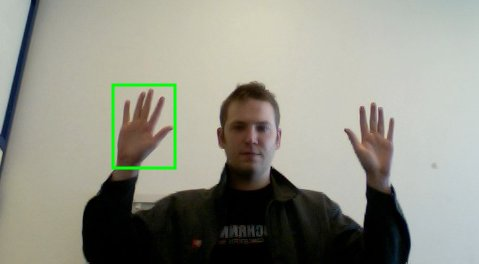
\includegraphics[width=0.45\linewidth]{figures/template/good.jpg}}
\hspace{0.03\linewidth}
\subfloat[result of template search]{\label{fig:template_occlusion}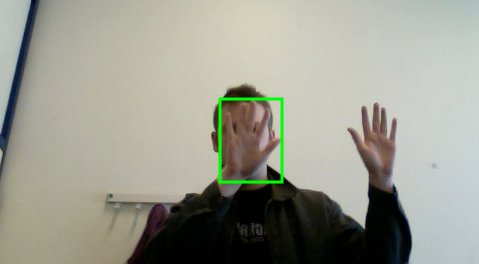
\includegraphics[width=0.45\linewidth]{figures/template/occlusion.jpg}}
\end{center}
\caption{Example of template search}
\label{fig:templatesearch}
\end{figure}

\autoref{fig:templatesearch} shows a test setting of a template search. In the left image The left hand was found using the skin model. In the second frame the hand cannot be found, because it is occluding the face and using the skin model approach the hand will be labeled as face. Using a template search the hand can still be tracked.


\section{Discussion}

\begin{figure}[htbp]
\center{}
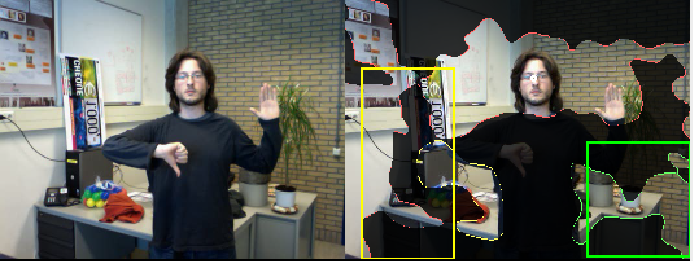
\includegraphics[width=0.8\linewidth]{figures/fail.png}
\caption{Example of failed segmentation}
\label{fig:fail}
\end{figure}


A parameterless method of going from the probabilistic domain to the binary domain is adaptive thresholding.

The face detection is one of the most expensive operations in the processing chain. Since in a single shot movie usually a face doesn't move fast, a number of frames can be skipped which will free more computational time for other operations.


